
\documentclass[polish,12pt]{aghthesis}

\usepackage[utf8]{inputenc}
% \usepackage{polski}
% \usepackage[polish]{babel}
\usepackage{url}
\usepackage{hyperref}
\usepackage{pgffor}
\usepackage{amsmath}

\def\sectionautorefname{rozdziale}

\usepackage{natbib}
\usepackage{keyval}
\usepackage{usebib}
\bibliographystyle{abbrv}
\bibinput{bibliografia}

\usepackage{listings}
\lstset{tabsize=4, frame=tb, numbers=none}

\usepackage{tabulary}

\usepackage{pdfpages}

\graphicspath{{images/}}

\author{Dawid Szmigielski, Radosław Chamot, Michał Liszcz}

\title{Genetyczny algorytm przydziału autobusów w komunikacji miejskiej}

\supervisor{prof. dr hab. inż. Robert Schaefer}

\date{2015}

\begin{document}

\maketitle
\newpage

\tableofcontents
\newpage


%% section 1 %%%%%%%%%%%%%%%%%%%%%%%%%%%%%%%%%%%%%%%%%%%%%%%%%%%%%%%%%%%%%%%%%%

\section{Wprowadzenie} \label{sec:intro}
Problem optymalizacji sieci transportu miejskiego jest tematem licznych badań. Zapotrzebowanie na transport publiczny stale rośnie. Przewoźnicy dążą do minimalizacji kosztów operacyjnych a jednocześnie do zapewnienia pasażerom najwyższej jakości usług (minimalny czas oczekiwania na przystankach, duża częstotliwość kursowania na zatłoczonych liniach czy optymalne zapełnienie pojazdów). W tej pracy przedstawiamy własną propozycję rozwiązania problemu przydziału pojazdów komunikacji miejskiej do wyznaczonych tras.

\subsection{Opis problemu}
Poszukujemy optymalnego przydziału pojadzów komunikacji miejskiej do ustalonych tras linii. Linie łączą przystanki. Na odcinkach między przystankami panuje stałe natężenie ruchu pasażerów. Ścisłe sformułowanie problemu znajduje się w \autoref{sec:solution}.

\begin{figure}[!htbp]
	\centering
	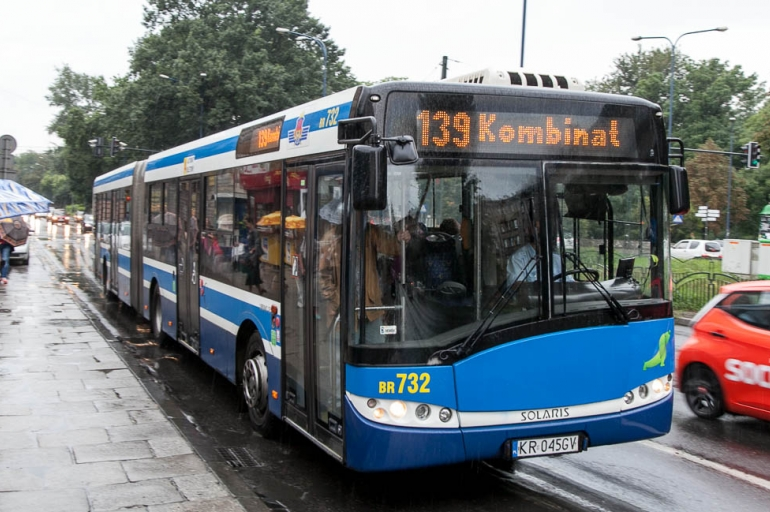
\includegraphics[width=0.9\textwidth]{351408454013_IMG_0581_770_512}
	\caption{Pojazd komunikacji miejskiej. Źródło: \textit{http://lovekrakow.pl}}
\end{figure}

\newpage



%% section 2 %%%%%%%%%%%%%%%%%%%%%%%%%%%%%%%%%%%%%%%%%%%%%%%%%%%%%%%%%%%%%%%%%%

\section{Przegląd rozwiązań}
Temat optymalizacji lini transportu miejskiego był poruszany w wielu pracach. Zaproponowano wiele różnych modeli, z różnymi ograniczeniami i różnymi kryteriami optymalizacji. Przedstawiamy tutaj najważniejsze spośród rozwiązań wykorzystujących algorytmy stochastyczne.

\paragraph{\cite{bib-large-scale}}
Przedstawia algorytm ustalania tras w sieci połączonych przystanków, z ograniczeniami uwzględniającymi długość trasy i ilość pojazdów (równoważne kosztowi operatora). Optymalizowana funkcja celu minimalizuje czas podróży użytkowników komunikacji między określonymi przystankami. Wykorzystuje symulowane wyżarzanie oraz \textit{fast descent (FD) search}.

\paragraph{\cite{bib-ant-colony}}
Przyjmuje następujące ograniczenia: określona maksymalna długość linii, minimalna liczba pasażerów jest wymagana do uruchomienia linii, pojemność linii musi być większa niż natężenie pasażerów. Wykorzystany algorytm to \textit{parallel ant colony algorithm} z wieloma koloniami mrówek jednocześnie wyszukującymi rozwiązania.

\paragraph{\cite{bib-transit-oriented}}
Autorska heurystyka optymalizująca przepływ pasażerów z użyciem standardowej macierzy OD (ang. \textit{origin-destination}).

\subsection{Pozostałe rozwiązania}
Inne podejścia, nie wykorzystujące algorytmów stochastycznych, to przykładowo:

\paragraph{\cite{bib-route-optimization}}
Minimalizacja kosztów operacyjnych i planowanie rozkładu połączeń z wykorzystaniem solwera CPLEX.

\paragraph{\cite{bib-theoretical-framework}}
Przeszukiwanie grafu połaczeń z uwzględnieniem rozkładu jazdy (\textit{time-dependent links}).

\newpage



%% section 3 %%%%%%%%%%%%%%%%%%%%%%%%%%%%%%%%%%%%%%%%%%%%%%%%%%%%%%%%%%%%%%%%%%

\section{Opis rozwiązania} \label{sec:solution}
Ten rozdział przedstawia naszą próbę rozwiązania problemu optymalnego przydziału pojazdów komunikacji miejskiej do wyznaczonych linii.

\subsection{Definicja problemu}
Sieć komunikacji miejskiej dana jest w postaci ciągu odcinków $R$, łączących przystanki. Każdy z takich odcinków charakteryzuje dodatnia liczba całkowita $r_i$, będąca natężeniem ruchu na tym odcinku (ilość pasażerów do przewiezienia w jednostce czasu).

W sieci komunikacji miejskiej istnieją ustalone trasy (linie). Zbiór wszystkich lini to $\mathcal{L}$. Linia $L_i$ jest ciągiem złożonym z indeksów kolejnych odcinków leżących na trasie tej linii.

\subsubsection{Dane wejściowe}
Na wejściu dana jest mapa sieci w postaci ciągu odcinków, oraz zbiór wszystkich linii autobusowych:

\begin{eqnarray}
R = (r_1, r_2, ..., r_n) \nonumber \\
\mathcal{L} = \{L_1, L_2, ..., L_m\} \\
L_i = (l_1^i, l_2^i, ..., l_k^i) \nonumber
\end{eqnarray}

\subsubsection{Dane wyjściowe}
Rozwiązaniem jest przypisanie każdej z $m$ linii $L_i$ dodatniej liczby autobusów $d_i$. Całkowita liczba autobusów jest ograniczona i nie można tej wartości przekroczyć. $m$-wymiarowy wektor rozwiązania:
\begin{equation}
D = (d_1, d_2, ..., d_m)
\end{equation}

\subsubsection{Optymalizacja}
Do każdej z linii należy przypisać pewną liczbę autobusów $d_i$ tak, aby zminimalizować:
\begin{itemize}
	\item liczbę pazażerów nieprzewiezionych (dopuszczamy przypadek że autobus nie zmieści wszystkich pasażerów)
	\item liczbę pustych miejsc w autobusie (większe zapełnienie autobusu zwiększa zysk przewoźnika)
\end{itemize}

Przyjmujemy jednakową pojemność wszystkich autobusów - każdy może przewieźć $Q$ pasażerów. Algorytm można jednak łatwo rozszerzyć o niejednorodne środki komunikacji.

Przy powyższych oznaczeniach wartość rozwiązania (funkcja celu) wyraża się poprzez:
\begin{equation}
value(D) = \sum_{r_i \in R}|
	r_i - \sum_{L_j \in \mathcal{L}}\sum_{l_n^j \in L_j} \delta_{l_n^j}^i d_j Q
| 
\end{equation}

\subsection{Algorytm}
Zaproponowane rozwiązanie to genetyczny algorytm ewolucyjny.

\subsubsection{Schemat ewolucji}
Na początku tworzona jest populacja losowych osobników. Następnie, wykonywane jest $N$ iteracji:

\begin{lstlisting}[language=Python]

# S is population size
population = create_random_population(S)

best = None

for _ in range(N):

	population = population.order_by( D => value(D) )
	new_population = []
	
	# take 25% best individuals
	new_population += population.take(S/4)
	
	# generate 25% new
	new_population += create_random_population(S/4)
	
	# randomly crossover and mutate 50%
	new_population += population.sliding(2)
	.map( (p1, p2) => mutation( crossover(p1, p2) ) )
	
	population = new_population
	
	new_best = population.min_by( D => value(D) )
	
	if best == None || best > new_best :
		best = new_best
		
# best contains solution with minimal value
\end{lstlisting}

\subsubsection{Kodowanie}
Z każdym z osobników związane jest rozwiązanie - wektor dodatnich liczb $D$ określających ilość autobusów $d_i$ na danej linii $L_i$. Suma wszystkich elementów tego wektora nie może przekroczyć maksymalnej liczby dostępnych autobusów.

\subsubsection{Krzyżowanie}
W wyniku krzyżowania dwóch osobników $P1$ oraz $P2$ może powstać nowy osobnik $P3$ lub procedura krzyżująca może zwrócić jednego z osobników $P1$ lub $P2$. Do krzyżowania dochodzi z ustalonym prawdopodobieństwem. Wtedy, zgodnie z rozkładem Bernouliego losowana jest maska określająca które części genotypu będą pochodzić od osobnika $P1$ a które od $P2$.

Dodatkowym warunkiem na odziedziczenie części genotypu jest przypisanie mniejszej liczby autobusów na danej linii przez rodzica.

\begin{lstlisting}[language=Python]
def crossover(P1, P2):

	if rand(0, 100) > crossoverProbability:
		return P1 if value(P1) < value(P2) else P2
	else:
	
		P3 = new_individial()
	
		for i in range(P1):
			P3[i] = P1[i]
				if P1[i] < P2[i] && bernoulli() == 1
				else P2[i]
				
		return P3

\end{lstlisting}

\subsubsection{Mutacja}
Osobniki powstałe w wyniku krzyżowania są (z niewielkim prawdopodobieństwem, 2\%) poddawane mutacji. W procesie mutacji losowana jest maska określająca które elementy genotypu będą zmieniane. Nowa wartość jest losowana w taki sposób, by nie przekroczyć górnego ograniczenia na liczbę autobusów.

\begin{lstlisting}[language=Python]
def mutation(P):

	if rand(0, 100) > 2:
		return P
	else:
	
		# generate mutation mask (bernoulli distribution)
		fields_to_change = ...
	
		for i in random_shuffle(fields_to_change):
			# use safe values for min and max
			P[i] = random(min, max)
	
		return P
	
\end{lstlisting}

\newpage



%% section 4 %%%%%%%%%%%%%%%%%%%%%%%%%%%%%%%%%%%%%%%%%%%%%%%%%%%%%%%%%%%%%%%%%%

\section{Wyniki}
Blah blah.

\newpage



\nocite{bib-transit-oriented}

\bibliography{bibliografia}
\newpage

\listoffigures
\newpage

\end{document}
